\documentclass[12pt]{article}
\usepackage{times}
\usepackage{geometry}
\usepackage[english]{babel}
\usepackage[utf8]{inputenc}
\usepackage{fancyhdr}
\usepackage{graphicx}
\usepackage{titlesec}


\setlength{\headheight}{15.2pt}
\setcounter{secnumdepth}{4}

\titleformat{\paragraph}
{\normalfont\normalsize\bfseries}{\theparagraph}{1em}{}
\titlespacing*{\paragraph}
{0pt}{3.25ex plus 1ex minus .2ex}{1.5ex plus .2ex}

\rfoot{Pg: \thepage}

\geometry{
   a4paper,
   left = 20mm,
   top = 20mm,
}
\begin{document}
\thispagestyle{empty}

\section*{}
{\LARGE\makebox[\textwidth]{\textbf{KATHMANDU UNIVERSITY}}}

\centerline{Department of Computer Science and Engineering}
\centerline{Dhulikhel,Kavre}
\begin{figure}[h]
    \centerline{
\includegraphics[width=50.546mm,height=50.546mm]{KU_Logo.png}}
\end{figure}

\centerline{\textbf{A Project Report}}
\centerline{on}
\centerline{\underline{\textbf{"Distributed Library"}}}

\vspace*{12mm}

\centerline{\textbf{[Code No. : COMP 207]}}
\centerline{(For partial fulfillment of 2nd Year/ 4th Semester in Computer Science)}

\vspace*{10mm}

\centerline{\textbf{Submitted by}}

\centerline{\textbf{Rabin Bhandari(Roll No. 6)}}
\centerline{\textbf{Susil Raj Neupane(Roll No. 39)}}
\centerline{\textbf{Aayush Pokharel(Roll No. 43)}}
\centerline{\textbf{Bijen Rayamajhi(Roll No. 48)}}


\vspace*{16mm}


\centerline{\textbf{Submitted to}}
\centerline{\underline{\textbf{Project Cordinator}}}
\centerline{\textbf{Pranita Karki}}
\centerline{\textbf{Dept of Computer Science and Engineering}}
\vspace*{10mm}

\centerline{\textbf{Submission Date: 6th May, 2022}}

\clearpage
\thispagestyle{empty}
\vspace*{10mm}
\centerline{\textbf{\Large{Bonafide Certificate}}}
\vspace*{30mm}
\centerline{\textbf{This project work on “Distributed Library” is the}} 
\vspace*{2mm}
\centerline{\textbf{bonafide work of}}
\vspace*{2mm}
\centerline{\textbf{"}}
\centerline{\textbf{Aayush Pokharel(Roll No. 43)}}
\centerline{\textbf{Susil Raj Neupane(Roll No. 39)}}
\centerline{\textbf{Rabin Bhandari(Roll No. 6)}}
\centerline{\textbf{Bijen Rayamajhi(Roll No. 48)}}
\centerline{\textbf{"}}
\vspace*{2mm}
\centerline{\textbf{who carried out the project work under my supervision.}}
\vspace*{80mm}
\textbf{Project Supervisior}
\\\\
\\\\
\textbf{-----------------------------------------------}
\vspace*{2mm}
\\
\textbf{Name: Amrit Dahal}
\vspace*{2mm}\\
\textbf{Academic Designation: Lecturer}
\vspace*{2mm}\\
\textbf{Dept. of Computer Science and Engineering}

\clearpage
\pagenumbering{roman}


\section{Acknowledgement}
\vspace*{5mm}

We wish to express our sincere thanks to the Department of Computer Science and 
Engineering for including the COMP 207 project into our curriculum. We would 
like to express our heartfelt gratitude to our project coordinator 
Ma’am Pranita Karki and our supervisor Mr. Amrit Dahal for their regular 
guidance and encouragement throughout the project. Taking this opportunity, we would 
like to thank all those individuals who directly or indirectly helped us in making 
this project successful, one be it by encouraging us throughout the project or 
else through their valuable suggestions which we have tried our best to assimilate 
within our work.

\clearpage

\section{Abstract}
The project ‘Decentralized Library’ proposal is drafted to meet the prerequisites 
to partially fulfill the COMP 207 course offered by the Department of Computer 
Science and Engineering at Kathmandu University. This project is designed to 
overcome the lack  of large public Libraries in Nepal and the economic burden 
it puts on students as well as other people who have to buy too many books due to 
lack of proper book lending facilities. The proposed App will act as a search 
engine platform which will catalog books near the users and facilitate exchange of 
books between its users. It will include displaying a curated selection of books 
available for exchange as per user-selected genres along with a list of books the 
users are searching for. There would be a chat feature to facilitate the exchange 
along with an embed map and GPS for ease of setting exchange spots.

We, the involved project members, have decided to create a WebApp that uses 
REST API framework in accomplishing this project by using Python and TypeScript 
as the main programming language. We will be using the Django(Python) framework 
for backend and Angular(TypeScript) framework for frontend.
\\\\
\textbf{Keywords:} TypeScript, WebApp, frontend, backend, GPS

\clearpage
\section{List of Symbols}

\clearpage
\section{Abbreviation}
\begin{itemize}
    \item \textbf{CSS : Cascading Style Sheets}
    \item \textbf{HTML : Hyperlink Text Markup Language}
    \item \textbf{SQL : Structured Query Language}
    \item \textbf{CLI : Command Line interface}
    \item \textbf{UI : User Interface}
    \item \textbf{SCSS : Syntactically Awesome Styles Sheets}
    \item \textbf{API : Application Programming Interface}
    \item \textbf{GUI : Grpahical User Interface}
    \item \textbf{JWT : Java Web Token}
    \item \textbf{ER : Entity-Relation}
    \item \textbf{BLOB : Binary Large Object}
    \item \textbf{vw : Wiew Width}
    \item \textbf{REST : Representational State Transfer}
\end{itemize}

\clearpage
\thispagestyle{empty}
\tableofcontents

\clearpage
\thispagestyle{empty}
\listoffigures

\clearpage
\pagenumbering{arabic}
\section{CHAPTER 1: INTRODUCTION}

\subsection{Background}
Even in today’s time the majority of people still prefer to read paper books. For 
this they buy books, read them and afterwards it’s left gathering dust in the 
shelves. Buying books is a costly endeavor when a devoted reader goes through a 
double digit number of books in a span of a few months. This leads to both an 
economic burden as well as a space problem.
\\
Borrowing from the Library could easily solve this problem but sadly Libraries are 
an infrastructure that is in poor quality in the context of Nepal. Mostly all the 
Libraries are either a personal one or an institutional one. With institutional 
Library being mostly of Schools and University where course books are the focus and 
personal Libraries are personal collections of an individual. It is very hard to 
borrow books and people need to either buy books or read online pirated transcripts.
\\
Therefore our proposed app comes into play as a platform to lend and borrow books. 
With a peer to peer exchange facility, the physical need to house books is 
circumvented and an active local community of book readers could potentially arise.

\vspace*{5mm}
\subsection{Objectives}
The main objective of this project is to make a virtual decentralized library where 
people can exchange books with each other and actually deploy it on the internet.
\\\\
Besides, the other objectives are listed below:
\begin{itemize}
    \item To circumvent the physical need to store books in a central location.
    \item To have a robust website with proper validators.
    \item To provide a book cataloguing service.
    \item To lighten the economic burden of buying books as well as provide an alternative to book hoarding.
    \item To promote a book reading culture.
\end{itemize}

\vspace*{5mm}
\subsection{Motivation and Significance}
Our project is particularly inspired by the lack of fictional books in Kathmandu 
University Central Campus Library. Furthermore this is a situation that is prevalent 
in other educational institutions as well. As students the economic burden of buying 
new books every time is a heavy burden and the lack of any platform to properly share 
books is a situation that we the team members have personally experienced.

Furthermore the site Goodreads; a books cataloging website; is a primary point of 
inspiration in tackling this project. A platform that works on a local level to 
provide an exchange catalog of locally available books is the main draw for the 
team to work in this project.

\clearpage

\section{CHAPTER 2: RELATED WORKS}
There are similar sites that provide book cataloguing,lending or buying service. Some of such sites that
are in use are:
\\\\
Some of such sites that are in use are:

\subsection{GoodReads}
\begin{figure}[h]
    \centerline{
\includegraphics[width = 90mm]{goodreads.jpg}}
    \caption{GoodReads}
    \label{fig}
\end{figure}
One of the primary experiences for this project, Goodreads is an American website 
which provides book cataloging features and is one of the most widely used services 
among book readers to keep track of books that they have read, are looking to read 
and new upcoming books.
\vspace{10mm}
\clearpage
\subsection{Scribd}
\begin{figure}[h]
    \centerline{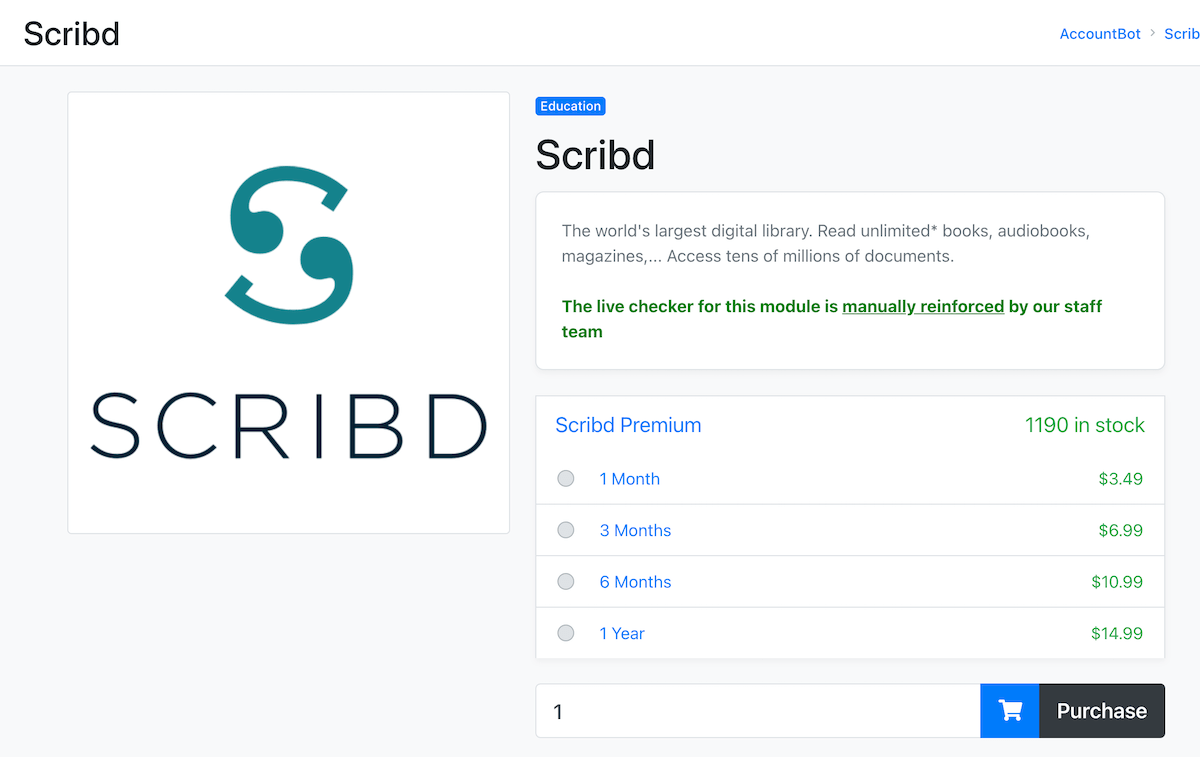
\includegraphics[width = 90mm]{scribd.png}}
    \caption{Scribd}
    \label{fig}
\end{figure}
An e-book and audio book subscription service, Scribd has been referred to as the 
”Netflix of Books”. For a small subscription charge, Scribd grants access to a 
large repository of e-books and audio books.
\clearpage

\section{CHAPTER 3: DESIGN AND IMPLEMENTATION}
\subsection{Architectural Design}
\subsubsection{Flowchart}
\begin{figure}[h]
    \centerline{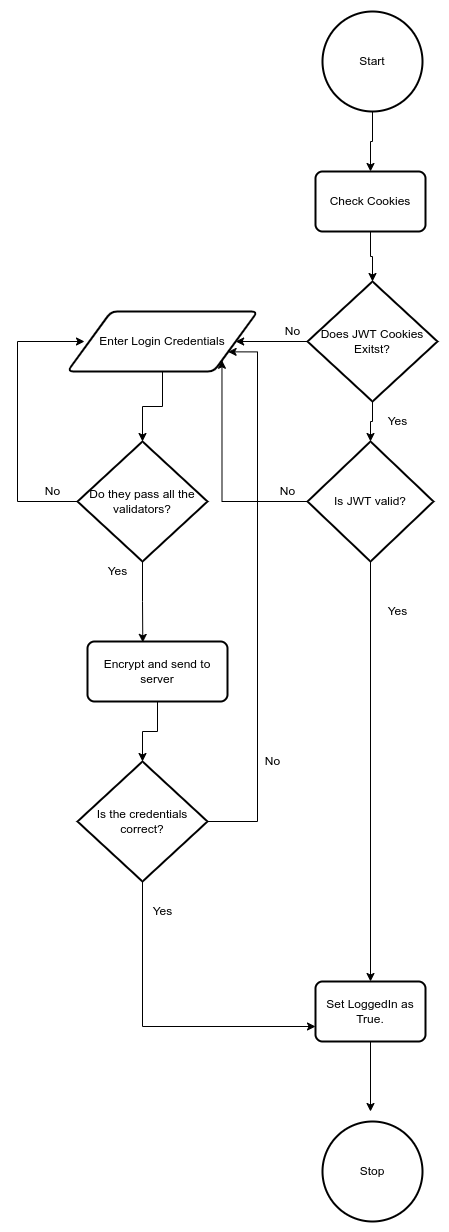
\includegraphics[height = 160mm]{login.drawio.png}}
    \caption{Log In Flowchart}
    \label{fig}
\end{figure}
\begin{figure}[h]
    \centerline{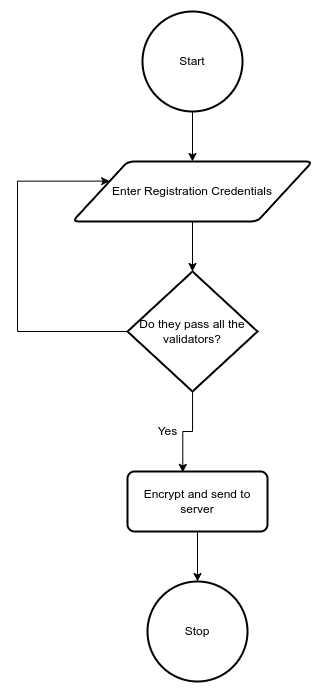
\includegraphics[width = 50mm]{register.drawio.png}}
    \caption{Register Flowchart}
    \label{fig}
\end{figure}
\begin{figure}[h]
    \centerline{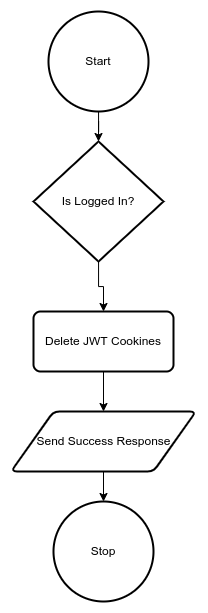
\includegraphics[width = 50mm]{logout.drawio.png}}
    \caption{Logout Flowchart}
    \label{fig}
\end{figure}


\clearpage
\subsection{System Requirement Specification}
\subsubsection{Software Requirements:}
\begin{itemize}
    \item \textbf{Front End Tools}
        \begin{itemize}
            \item The UI is created using TypeScript,CSS and HTML.
            \item Development Tools : Angular framework
        \end{itemize}
    \item \textbf{Back End Tools}
        \begin{itemize}
            \item The backend is created using Python.
            \item SQL or No-SQL database will be used for storing data.
            \item Development Tools : MySQL, Django
        \end{itemize}
\end{itemize}

\subsubsection{Hardware Requirements:}
\begin{itemize}
    \item Compatibility: (Development) Compatible with all PCs able to run python and AngularCLI.
    \item Compatibility: (Deployment) Compatible with all servers capable of python hosting.
    \item Compatibility: (Usage) Compatible with all PCs able to run a modern Internet Browser.
\end{itemize}

\vspace*{10mm}
\textbf{Python :} A dynamically typed multi paradigm general purpose programming language.
\\\\
\textbf{SQL :} Structured Query Language, an standardized programming used to maintain Relational
databases as well as perform operations on the data in them.
\\\\
\textbf{Django Framework :} An open source web framework written in python that follows model-templates-
view architecture.
\\\\
\textbf{Angular CLI :} The Command line interface of popular frontend web development framework Angular
which is maintained by Google.

\clearpage
\section{CHAPTER 4: DISCUSSION AND  ACHIEVEMENT}

\subsection{Methodology}
The whole process of developing the software has been divided into following aspects:
\begin{itemize}
    \item Research and study
    \item UI Design and prototyping
    \item Core programming
    \item Program Testing
    \item Documentation
\end{itemize}

\subsubsection{Research and Study}
This project being the first of the kind we have ever done, we decide to choose a subject matter that we clearly know and have experience with i.e. Database focused application . 

We have interacted with the various software/sites mentioned above in chapter 2 on a semi-regular basis and have experienced its strength 
and pitfall. We are trying to provide a grass root service that we hope will take wide spread adoption.

\subsubsection{UI design and Prototyping}
The initial designs are sketched on A4 papers by our members and shared on group chat for peer review and then we use figma to design test the look of our UI before adding any frontend code to make it in CSS or SCSS.

\subsubsection{Core Programming}
The most amount of project time was spent in this stage. We are using the Python language to write our backend program. The Angular framework provides the necessary tools to create 
the GUI. Django (WhiteNoise plugin) is being used to serve the static web pages to the web and Django Rest API provides get, put and update APIs to manipulate data for LogIn/Register 
(Using JWT) or to update the various other data models.


\paragraph{Issues Encountered}
\begin{itemize}
    \item \textit{\textbf{Team Members catching COVID-19}}\\
        After the initial design phase of the the project was complete. Half the members of the development caught COVID-19 and work was halted. This went on for some time and the issue was compounded by other academic responsibilities due to which there was periods of inactivity during development phase.
    \item \textit{\textbf{Adapting the frontend code with framework}}\\
        Due to part of the team members only having learned vanilla HTML and CSS, it was confusing to adapt the code written by multiple parties to comply with single page application code. 
        one prominent example was of using anchor tag for navigation with href and Routerlink.
    \item \textit{\textbf{Routing issue}}\\
    Due to Django and Angular both providing web page routing,initially it was confusing to separate the frontend routing and backend routing. The web pages' view routing were done in angular along with error handling whereas API endpoint routing was done in Django.
    \item  \textit{\textbf{Managing Django Migrations}}\\
    We initially made some IR models and went to code the application as per the design schema but managing multi-valued attributes and foreign key constraints was difficult and there was a lot of deviation to the initial design. Furthermore, due to these deviations, 
    the data needed to be entered multiple times in the database and we had to rollback the migrations and redo them. This causes issues like accidental deletion of wrong migrations and a deadlock in generation of new migrations. This had us repeat this procedure.
    \item  \textit{\textbf{Image Storage}}\\
        Initially we had thought to store images as BLOB objects after they were standardized in resolution through manipulation via the Python Image Library in the database but the Django framework calls for the files to be stored in the directory and it was difficult to store them. Idea to introduce MongoDB for image file storage was introduced but due to time and code complexity of working multiple databases, it was passed over and images were simply stored in a directory.
    \item \textit{\textbf{Geo-location Features}}\\
    Initially our application was supposed to have Geo-location ability via Open Streets API but due to our limited understanding of converting the Geo=location coordinates to get a radius and the query getting more and more complex with each API. We decided to forgo the Geo-location.
    \item \textit{\textbf{Brainstorming features to be added}}\\
        Initially the project was on different trajectory and due to amount of time invested, team members were locked in a certain direction. The team was a newly formed team and it took some time for internal communication between members to be smooth.
    \item \textit{\textbf{Database Loading and Exporting}}\\
        MySQL database wasn't being loaded via a CSV file and was saying that local files from only certain directory could be loaded or exported to. The problem was that the default specified directory was within root directory and superuser privilege was necessary to even access the directory further more we could change the directory as it required various system setting for MySQL service to be edited as per stack over flow which we didn't understand.
    \item \textit{\textbf{Difficulty in getting domain from mercantile host master}}\\
        Despite filling forms properly multiple times to get a domain, mercantile host master always denied the request claiming insufficient documents. Thus domain and hosting had to be bought from Tech Himalaya.
\end{itemize}
\subsubsection{Program Testing}
Unit testing was done as soon as we completed the code of a single widget to check its functioning properly. This was repeated multiple times during the development 
period to create a robust system and once the core programming is completed, alpha testing was done to find different types of bugs or ill optimised issues.
\paragraph{Bugs found}
\begin{itemize}
    \item The CSS absolute units (vw and vw) were making the layout of the have horizontal scroller even when it wasn't necessary.
    \item Chat API were not loading the JSON properly.
    \item The View was not updating when the database was updated and was needing server restart.
\end{itemize}
\paragraph{Bugs debugged}
\begin{itemize}
    \item Relative units percentage was chosen to make the layout.
    \item Single class based API for chat was broken down and expanded to make 3 different classes, one for inital loading,one to update the gui and one to send messages.
    \item It was an error caused due to the function only being called on intialization. It's function call was changed to call everytime there was a update via obserables.
\end{itemize}
\clearpage
\subsection{Features}
We wanted to make this a deployable project so instead of a large project, we tried to make the code robust with a lot of validators and proper work.

\subsubsection{FrontEnd}
\begin{itemize}
    \item Single Page application with Angular routing for a smooth transition between views without reloading the web page.
    \item Encryption of the Login/Register Information on front end to deny packet sniffing threats.
    \item Catalogue as per genres.
    \item Catalogue as per newly added items.
    \item Catalogue as per author.
    \item Chat box for peer to peer interaction with other book owners registered in the site.
    \item Search bar according to genres, newly added items and author.
\end{itemize}
\subsubsection{Backend}
\begin{itemize}
    \item Actual Deployment 
    \item JWT based authentication
    \item MySQL connection via Django Library
    \item Class based Restful API. 
\end{itemize}

\clearpage

\section{CHAPTER 5: CONCLUSION AND RECOMMENDATION}
With the constant supervision of the supervisor and hard work of team members, the project is finally complete. After this project we believe our team is 
ready to tackle more sophisticated projects in the future.

\subsection{Limitations}
\vspace*{5mm}
The program has the following limitations:
\begin{itemize}
    \item \textit{\textbf{No Geo-location}}\\
        The project was initially designed to show recommendations based on user location but due to the Geo-location queries' complexity, it was changed to display all the available content.
    \item \textit{\textbf{Lack of channels in chat}}\\
        We tried to actually have channels in chat so two users could connect with each other and then their messages would get saved in the database but we found it incompatible to use channels with REST APIs so the whole chat was remade using REST APIs for backend logic and storage where as Angular consumable was used to update the UI. 
\end{itemize}
\vspace*{5mm}
\subsection{Further Enhancements}
\vspace*{5mm}
The following action could be undertaken to improve the program.
\begin{itemize}
    \item \textit{\textbf{Making a proper Geo-location service application}}\\
        None of the team members had any experience with using the Geo-location API and the complex queries which required trigonometric functions to work. Therefore, as we would actually like to launch this service, we would like to spend more time on learning about latitudes and longitudes and properly add the functionality.

    \item \textit{\textbf{Making the app single language}}\\
        Due to the confusing stacks of programming languages, we wish to either shift to an expression express server or make it a server side Django application.
    \item  \textit{\textbf{Making a Mobile App}} 
        If possible, in next semester we would like to explore mobile apps and convert this application to either work as a Hybrid app or a web view app.
\end{itemize}
\clearpage

\section{References}
\thispagestyle{empty}
Goodreads. Goodreads. (2022). Retrieved from\\
https://www.goodreads.com/.
\\\\
Subscribe to the world's largest digital library. Scribd. (2022). Retrieved from\\
https://www.scribd.com/.
\\\\
The web framework for perfectionists with deadlines | Django. Djangoproject.com. (2022).\\
Retrieved from https://www.djangoproject.com/.
\\\\
Angular. Angular.io. (2022). Retrieved from\\
https://angular.io/cli.
\\\\
Typescriptlang.org. (2022). Retrieved from\\
https://www.typescriptlang.org/.
\\\\
MySQL. Mysql.com. (2022). Retrieved from\\
https://www.mysql.com/.



\clearpage
\thispagestyle{empty}
\section{Appendix}
\thispagestyle{empty}
\begin{figure}[h]
    \centerline{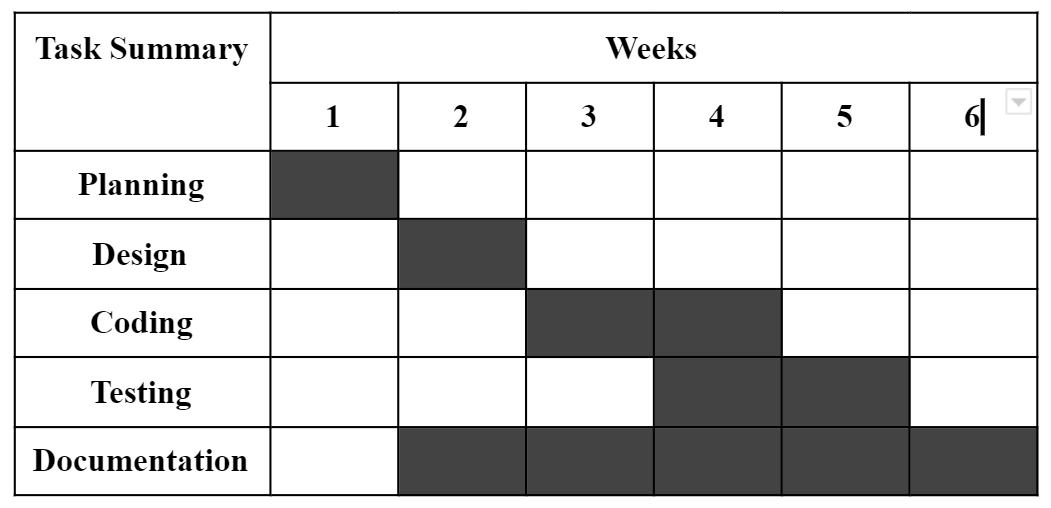
\includegraphics[width = 190mm]{chart.png}}
    \caption{Gantt Chart}
    \label{fig}
\end{figure}
\rightline{\underline{\textbf{Index}}}
\begin{figure}[h]
    \rightline{
\includegraphics[width=15mm,height=15mm]{box.png}}
\end{figure}
\rightline{\underline{\textbf{Task Completed}}}

\end{document}
